\documentclass{beamer}

\usepackage{hyperref}
\hypersetup{
  colorlinks = true
}
\usepackage[utf8]{inputenc}
\usepackage{amsmath}
\usepackage{amssymb}

% beamer
\setbeamertemplate{navigation symbols}{}

% macros
\DeclareMathOperator*{\argmax}{arg\,max}
\DeclareMathOperator*{\argmin}{arg\,min}

% Information to be included in the title page:
\title{ECE 590D-001, Reinforcement Learning at Scale}
\author{Jay Hineman, Ph.D.}
\institute{Geometric Data Analytics}
\date{2020}
 
 
\begin{document}
\frame{\titlepage}
\begin{frame}
  \frametitle{Mathematical details (restated) \cite{Sutton2018}}
  {\bf Following Sutton and Barto \cite{Sutton2018}}
  \begin{itemize}
  \item $t=\text{time/iteration}$, $s, S_t \in \mathcal{S} = \text{states}$, $a, A_t \in \mathcal{A}(s) = \text{actions at state}$, $r, R_{t+1} \in \mathbb{R} = \text{rewards}$,
    $S_0, A_0, R_1, S_1, A_1, R_2, S_2, A_2, R_3, \ldots = \text{trajectory}$
  \item $\text{transition function} = p(s', r'| s, a) := \text{Prob}\{S_t = s', R_t = r | S_{t-1} = s, A_{t-1} = a\}$
  \item {\bf probability fact:} $\sum_{s',r} p(s',r | s, a) = 1$ for all $s \in \mathcal{S}, a \in \mathcal{A}(s)$
  \item {\bf return and discounted return:} $G_t = R_{t+1} + R_{t+2} + R_{t+3} + \cdots + R_{T}$ and $G_t = R_{t+1} + \gamma R_{t+2} + \gamma^2 R_{t+3} + \cdots$
  \item {\bf ((board work))} from \cite{Sutton2018}
  \end{itemize}
\end{frame}


\begin{frame}
  \frametitle{Mathematical specification of value and action-value (restated)}
  \begin{equation}
    \begin{aligned}
      q_\pi(s) &= \mathbb{E}_\pi[G_t|S_t = s, A_t = a] \\
      &= \mathbb{E}_\pi [\sum_{k=0} \gamma^k R_{(t + 1) + k} | S_t = s, A_t = a ], s \in \mathcal{S} \\
      &= \text{Value of $s$ given the policy $\pi$} \\
      v_\pi(s) &= \mathbb{E}_\pi[G_t|S_t = s] \\
      &= \mathbb{E}_\pi [\sum_{k=0} \gamma^k R_{(t + 1) + k} | S_t = s ] \\
      &= \text{action-value or $q$-value of $s,a$ given the policy $\pi$}
    \end{aligned}
  \end{equation}
  \begin{itemize}
  \item {\bf ((board work))} on {\em Bellman equation} for $v_\pi$ from \cite{Sutton2018}
  \end{itemize}
\end{frame}

\begin{frame}
  \frametitle{Bellman Equation}
  \begin{itemize}
  \item {\bf Bellman equation} for value function: $v_\pi(s) = \sum_a \pi(a|s)
\sum_{s', r} p(s',r|s,a) [r + \gamma v_{\pi} (s')$
  \item {\bf Exercise:} Convince yourself, perhaps by making a more explicit
    notation, that (3.14) in \cite{Sutton2018} is simply an expectation.

  \item {\bf Exercise:} Determine the Bellman equation for action-value. See Exercise
    3.17 \cite{Sutton2018}.
  \end{itemize}
\end{frame}

\begin{frame}
  \frametitle{Optimal Policies and Value functions \cite{Sutton2018}}
  \begin{itemize}
  \item {\em Solving a reinforcement learning task means, roughly, finding a
      policy that achieves a lot of reward over the long run}
  \item Since we can establish a partial ordering of policies we can talk about
    optimality: {\em A policy $\pi$ is defined to be better than or equal to a
      policy $\pi'$ if its expected return is greater than or equal to that of $\pi'$
      for all states. In other words, $\pi \geq \pi'$ if and only if $v_\pi(s) \geq
      v_{\pi'} (s)$ for all $s \in \mathcal{S}$.}
  \item Denote (maybe non-uniquely) optimal policies by $\pi_*$. {\em They share the same
    value function and action-value function!}
  \end{itemize}
\end{frame}

\begin{frame}
  \frametitle{Optimal Policies and Value functions \cite{Sutton2018}}
  \begin{itemize}
  \item {\bf optimal state-value function:}
    \[ v_*(s) = \max_{\pi}v_{\pi}(s), \text{ for all } s \in \mathcal{S} \]
  \item {\bf optimal action-value function:}
    \[ q_*(s,a) = \max_{\pi} q_{\pi}(s,a), \text{ for all } s \in \mathcal{S}, a \in \mathcal{A}(s) \]
  \item Said another way:
    \[\pi_* = \argmax_{\pi} q_{\pi}(s,a) = \argmax_{\pi} v_{\pi}(s) , \text{ for all } s \in \mathcal{S}, a \in \mathcal{A}(s) \]
  \end{itemize}
\end{frame}

\begin{frame}
  \frametitle{Optimal Policies and Value functions \cite{Sutton2018}}
  \begin{itemize}
  \item {\bf Important identity:}
    \[q_*(s,a) = \mathbb{E}[R_{t+1} + \gamma v_*(S_{t+1}) | S_t = s, A_t = a] \]
  \item $v_*$ and $q_*$ must satisfy Bellman equations. {\em Because they are optimal
      ``value'' functions, their consistency condition can be written in a special form
      without reference to any specific policy}.
  \item {\bf Belleman optimality for $v_*$}
    \[v_*(s) = \max_a \sum_{s',r} p(s',r|s, a)[r + \gamma v_*(s'), s \in \mathcal{S}\]
  \item {\bf Belleman optimality for $q_*$}
    \[q_*(s,a) = \sum_{s',r} p(s',r|s, a)[r + \gamma v_*(s'), s \in \mathcal{S}, a \in \mathcal{A(s)}\]
  \end{itemize}
\end{frame}

\begin{frame}
  \frametitle{Optimal Policies and Value functions \cite{Sutton2018}}
  \begin{itemize}
  \item For finite MDPs, the Bellman optimality equation has a unique solution.
  \item Really, Bellman equations are (nonlinear) systems on for each state or state-action pair.
    {\em That means we can employ solution  methods for such equations (fixed point
      iteration, gradient descent, etc, {\bf if the dynamics are known}}
  \end{itemize}
\end{frame}

\begin{frame}
  \frametitle{Optimal Policy and Value function for Grid World, Example 3.8}
  \begin{itemize}
  \item In a future homework, we will compute similar value functions for gridworld
  \end{itemize}
  \begin{figure}
    \label{fig:gridworld-optimal}
    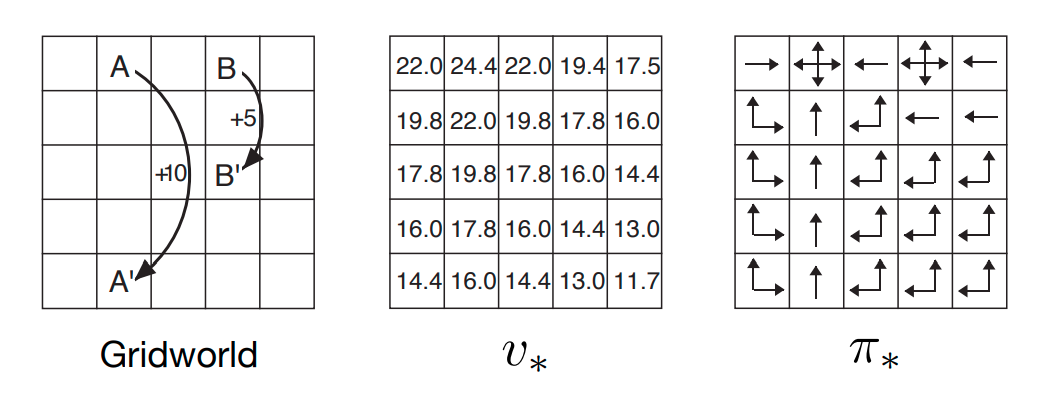
\includegraphics[width=\textwidth]{../images/sutton3_5_gridworld.png}
    \caption{A gridworld with optimal policy and value function, Example 3.8 \cite{Sutton2018}}
  \end{figure}
\end{frame}

\begin{frame}
  \frametitle{Spinning up's \href{https://spinningup.openai.com/en/latest/spinningup/rl_intro2.html}{Taxonomy}}
  \begin{figure}
    \label{fig:deep-rl-taxonomy}
    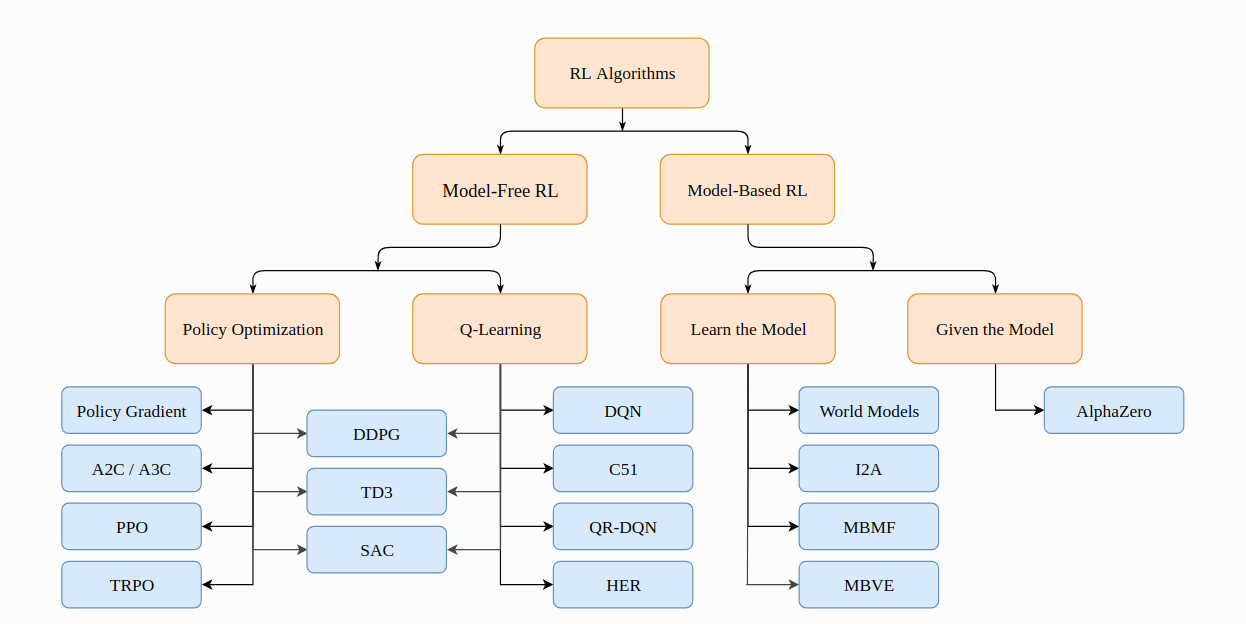
\includegraphics[width=\textwidth]{../images/spinup_rl_taxonomy.png}
    \caption{Non-exhaustive, but nice starting Taxonomy of (deep) RL methods. See also:
      \href{https://spinningup.openai.com/en/latest/spinningup/rl_intro2.html\#citations-below}{citations.}}
  \end{figure}
\end{frame}

\end{document}

% two column sample 
\begin{frame}
\frametitle{A frame}
  \begin{columns}[T]
    \begin{column}{.5\textwidth}
     \begin{block}{Your textblock}
% Your text here
    \end{block}
    \end{column}
    \begin{column}{.5\textwidth}
    \begin{block}{Your image}
% Your image included here
    \includegraphics[<options, e.g. width=\textwidth>]{<your image file>}
    \end{block}
    \end{column}
  \end{columns}
\end{frame}